% HiMCM 2025 Problem A --- Emergency Evacuation Sweeps
% Compile from the paper/ directory:
%   pdflatex himcm_paper.tex
% Figures are loaded from ../paper_figures/; tables use statistics
% computed from ../results/experiment_summary.csv (420 Monte Carlo runs).
\documentclass[12pt]{article}

\usepackage[margin=1in]{geometry}
\usepackage{amsmath,amssymb}
\usepackage{booktabs}
\usepackage{graphicx}
\usepackage{caption}
\usepackage{subcaption}
\usepackage{setspace}
\usepackage{enumitem}
\usepackage{array}
\usepackage[hidelinks]{hyperref}

\graphicspath{{../paper_figures/}{paper_figures/}{./}}
\hypersetup{
  pdftitle={HiMCM 2025 Problem A: Emergency Evacuation Sweeps},
  pdfauthor={Team XXXX}
}

\newcommand{\TeamNumber}{XXXX}
\newcommand{\Tclear}{T_{\mathrm{clear}}}
\newcommand{\tsvc}{t_{\mathrm{svc}}}
\newcommand{\tsw}{t_{\mathrm{sw}}}
\newcommand{\ttag}{t_{\mathrm{tag}}}
\newcommand{\whall}{v_{h}}
\newcommand{\vroom}{v_{r}}

\pagestyle{myheadings}
\markright{\TeamNumber \hfill HiMCM 2025 Problem A \hfill}

\title{\textbf{Coordinated Firefighter Sweeps under Time, Vulnerability,\\
and Spreading Hazards}\\[0.4em]
\large HiMCM 2025 Problem A --- Team \TeamNumber}
\author{}
\date{}

\begin{document}
\maketitle
\thispagestyle{empty}

\begin{center}
{\Large \textbf{Summary}}
\end{center}

We model emergency primary-search as a multi-agent covering process on a metric graph.
Rooms are leaves (or bays) that must be entered, visually confirmed, and tagged; hallways
and stairs are circulation edges with length in metres. Two firefighters clearing the
one-story office of Figure~1 admit an exact Split-Half lower bound
\begin{equation*}
  \Tclear^{\mathrm{SH}}
  = \frac{L/2}{\whall} + 3\tsvc
  = 145\,\mathrm{s}
\end{equation*}
when interior round-trips of depth \(D=8\,\mathrm{m}\) are folded into service time
\(\tsvc=45\,\mathrm{s}\). A deterministic scoring planner that walks room-access edges
instead of double-counting those round-trips clears the same building in
\(\Tclear=135\,\mathrm{s}\) (9 discrete steps of \(15\,\mathrm{s}\)).

The planner assigns idle agents the room \(r\) maximising
\begin{equation*}
  \mathrm{Score}(r)
  = -w_{\mathrm{dist}}\,d(a,r)
    -w_{\mathrm{hazard}}\,h(r)
    +w_{\mathrm{priority}}\,v(r)
    -w_{\mathrm{redundancy}}\mathbf{1}_{\mathrm{tgt}}
    -w_{\mathrm{tabu}}\mathbf{1}_{T_a}(r)
    +w_{\mathrm{mom}}M(a,r),
\end{equation*}
with a tenure-3 room tabu list and a same-hub momentum bonus to prevent edge-reversal
cycling on loopy graphs. Scaling to a three-floor daycare (18 rooms) and an open
warehouse (40 searchable bays) shows strictly decreasing clearance time as crew size
grows: daycare \(439.0\to 300.7\to 255.7\,\mathrm{s}\) for \(2,3,4\) firefighters;
warehouse \(424.7\to 333.0\to 262.3\,\mathrm{s}\) for \(3,4,5\) firefighters
(\(N=30\) identical ideal-condition replications). The steepest personnel marginal
return is the step to 3 firefighters in the daycare (\(\Delta\Tclear=138.3\,\mathrm{s}\))
and to 4 in the warehouse (\(\Delta\Tclear=91.7\,\mathrm{s}\)).
A graph-attention PPO policy trained for 200 office episodes (no fire) does
\emph{not} replace the timed planner: greedy decoding never fully clears
(\(0/30\)), while stochastic decoding fully clears \(20/30\) trials
(mean \(5.60\) of \(6\) rooms tagged; Table~\ref{tab:rl}). We therefore keep the
scoring planner as the operational baseline and treat GAT-PPO as a learned
covering heuristic on the unweighted graph.

Under a dynamic fire/smoke process with
\(P_{\mathrm{spread}}=1-(1-p_0)^{k}\) and smoke-front speed \(1.5\,\whall^{\mathrm{fire}}\),
full-building clearance never occurred in 210 smoke trials: graphs become disconnected
before every room is tagged. Vulnerable-population salvage (weighted rooms tagged before
abort) remains informative: about \(20\%\) in the office, \(16\)--\(27\%\) in the daycare
as crew grows, and \(32\)--\(53\%\) in the warehouse. We treat abort times as
\emph{not} clearance times, recommend thermal/tag sensors as information that would
enter \(h(r)\) and \(v(r)\), and report sensitivity of \(\Tclear\) and salvage to crew
size and hazard mode directly from \texttt{experiment\_summary.csv}.

\tableofcontents
\newpage

%----------------------------------------------------------------------
\section{Problem Clarification \& Verification Criteria}

\subsection{Restatement of the task}

HiMCM 2025 Problem~A asks how firefighters should \emph{sweep} a building so that every
occupiable space is confirmed empty (or a victim is found) as quickly as possible, under
realistic movement, tagging, crew coordination, and spreading hazards. The contest
statement decomposes the work into five requirements, which we map one-to-one onto
Sections~\ref{sec:req1}--\ref{sec:req5} of this paper:
\begin{enumerate}[leftmargin=1.6em,itemsep=0.25em]
  \item verification language and assumptions (this section);
  \item a closed-form solution of the Figure~1 office;
  \item a scalable multi-agent model on a daycare and a warehouse;
  \item fire, smoke, and sensor-aware adjustments;
  \item sensitivity and robustness of the recommendations.
\end{enumerate}

\subsection{Decision variables, parameters, and notation}
\label{sec:req1}

A building is an undirected graph \(G=(V,E)\) with edge lengths \(\ell_e\) in metres.
A subset \(R\subseteq V\) of nodes is \emph{searchable} (offices, classrooms, storage
bays). Firefighters \(a=1,\ldots,m\) start at exit nodes. Time is continuous within
discrete planning steps of length \(\Delta t\).

Core kinematic parameters (office geometry of Figure~1, used as the default scale) are
\[
  L=30\,\mathrm{m},\quad
  D=8\,\mathrm{m},\quad
  \whall=1.5\,\mathrm{m/s},\quad
  \vroom=0.8\,\mathrm{m/s},\quad
  \tsw=20\,\mathrm{s},\quad
  \ttag=5\,\mathrm{s}.
\]
Single-room service in the analytical model is
\begin{equation}
  \label{eq:tsvc}
  \tsvc
  = \frac{2D}{\vroom} + \tsw + \ttag
  = 45\,\mathrm{s}.
\end{equation}

\subsection{Verification criteria (what ``success'' means)}

A policy is evaluated on three observable, CSV-recorded criteria.
\begin{description}[style=nextline,leftmargin=1.1em]
  \item[Total sweep time \(\Tclear\).]
    The instant at which the last searchable node is tagged. If the crew deadlocks or
    hits a step cap, we record the abort clock but \emph{do not} interpret it as a
    completed sweep.
  \item[Vulnerable-population salvage \(\eta\).]
    Let \(v(r)\ge 0\) be a vulnerability weight (infants \(5\), nap rooms \(4.5\),
    classrooms \(3\), staff \(1\); office rooms default to \(1\)). Then
    \begin{equation}
      \label{eq:eta}
      \eta
      = \frac{\sum_{r\in R_{\mathrm{tagged}}} v(r)}{\sum_{r\in R} v(r)}
      \in [0,1].
    \end{equation}
  \item[Redundancy rate \(\rho\).]
    If firefighter trajectories enter searchable node \(r\) a total of \(c_r\) times,
    \begin{equation}
      \label{eq:rho}
      \rho
      = \frac{1}{|R|}\sum_{r\in R}\max(c_r-1,0).
    \end{equation}
\end{description}
A run is a \emph{full clearance} only when \(\eta=1\) and every \(r\in R\) is tagged.
All numerical claims below are computed from the 420-row file
\texttt{results/experiment\_summary.csv} (\(N=30\) Monte Carlo replications per
scenario \(\times\) crew size \(\times\) hazard mode).

\subsection{Assumptions}
\begin{enumerate}[leftmargin=1.4em]
  \item Agents share a common tagged-set (perfect radio); they do not re-clear a tagged
        room except via residual path geometry.
  \item Tagging occurs at the room node after a visual sweep of duration \(\tsw\).
  \item Fire renders a node impassable; smoke multiplies speed by
        \(\max(v_{\min},1-\beta\sigma)\) with \(\beta=0.4\) at full density \(\sigma=1\).
  \item No civilian counter-flow is simulated; vulnerability enters only through \(v(r)\).
  \item Warehouse racks are obstacles, not searchable interiors; searchable bays are
        aisle cells adjacent to racks.
\end{enumerate}

%----------------------------------------------------------------------
\section{Base Model: One-Story Office Analytical Solution}
\label{sec:req2}

\subsection{Graph of Figure~1}

The office is the 11-node hanging graph
\[
  E_W-H_1-H_2-H_3-E_E,
\]
with north rooms \(N_1,N_2,N_3\) and south rooms \(S_1,S_2,S_3\) attached to
\(H_1,H_2,H_3\). Door abscissae matching Figure~1 are
\(x_{H_1}=10\), \(x_{H_2}=15\), \(x_{H_3}=20\), \(x_{E_W}=0\), \(x_{E_E}=L=30\).

\subsection{Split-Half lower bound}

Two firefighters entering from opposite exits, each taking three rooms, cannot beat
the load-balance bound \(\max_i|\mathcal{R}_i|\ge 3\) nor the hallway covering bound
of \(15\,\mathrm{m}\) from an exit to the mid-door. Hence
\begin{equation}
  \label{eq:tsh}
  \Tclear^{\mathrm{SH}}
  = \frac{15}{\whall} + 3\tsvc
  = 10 + 135
  = 145\,\mathrm{s}
\end{equation}
(\(W_h=0\)). The realizing partitions are
\(\mathcal{R}_1=\{N_1,S_1,N_2\}\) and \(\mathcal{R}_2=\{N_3,S_3,S_2\}\), with
column-first routes
\begin{align*}
  F_1&: E_W\to N_1\to S_1\to N_2,\\
  F_2&: E_E\to N_3\to S_3\to S_2.
\end{align*}
Returning to an exit after the last tag adds another \(15/\whall=10\,\mathrm{s}\)
(\(\Tclear^{\mathrm{egress}}=155\,\mathrm{s}\)).

Smoke that cuts hallway speed by \(40\%\) replaces \(\whall\) by
\(\whall' =0.9\,\mathrm{m/s}\). Dual cross-check of the two centre rooms adds one
extra \(\tsvc\) after the meeting at \(x=15\), giving
\(\Tclear^{\mathrm{RV}}=15/\whall'+4\tsvc=196.67\,\mathrm{s}\) when \(\gamma=1\).

\subsection{Operational FSM versus the bound}

The implemented planner walks the \(8\,\mathrm{m}\) room-access edge as movement at
\(\vroom\), then spends \(\tsw+\ttag=25\,\mathrm{s}\) in place. That FSM therefore
does not add a second interior round-trip of \(2D/\vroom=20\,\mathrm{s}\) on top of
the access edge. Discrete-event simulation from both exits yields
\begin{equation}
  \Tclear^{\mathrm{sim}}=135.0\,\mathrm{s}
\end{equation}
(9 steps \(\times\) \(15\,\mathrm{s}\)), with tags at \(41.67\,\mathrm{s}\)
(\(N_1,N_3\)), \(86.67\,\mathrm{s}\) (\(S_1,S_3\)), and \(135\,\mathrm{s}\)
(\(N_2,S_2\)). The \(10\,\mathrm{s}\) gap relative to~\eqref{eq:tsh} is exactly the
accounting difference in interior travel, not a violation of the covering lower bound
on \emph{that} service model.

\begin{figure}[htbp]
  \centering
  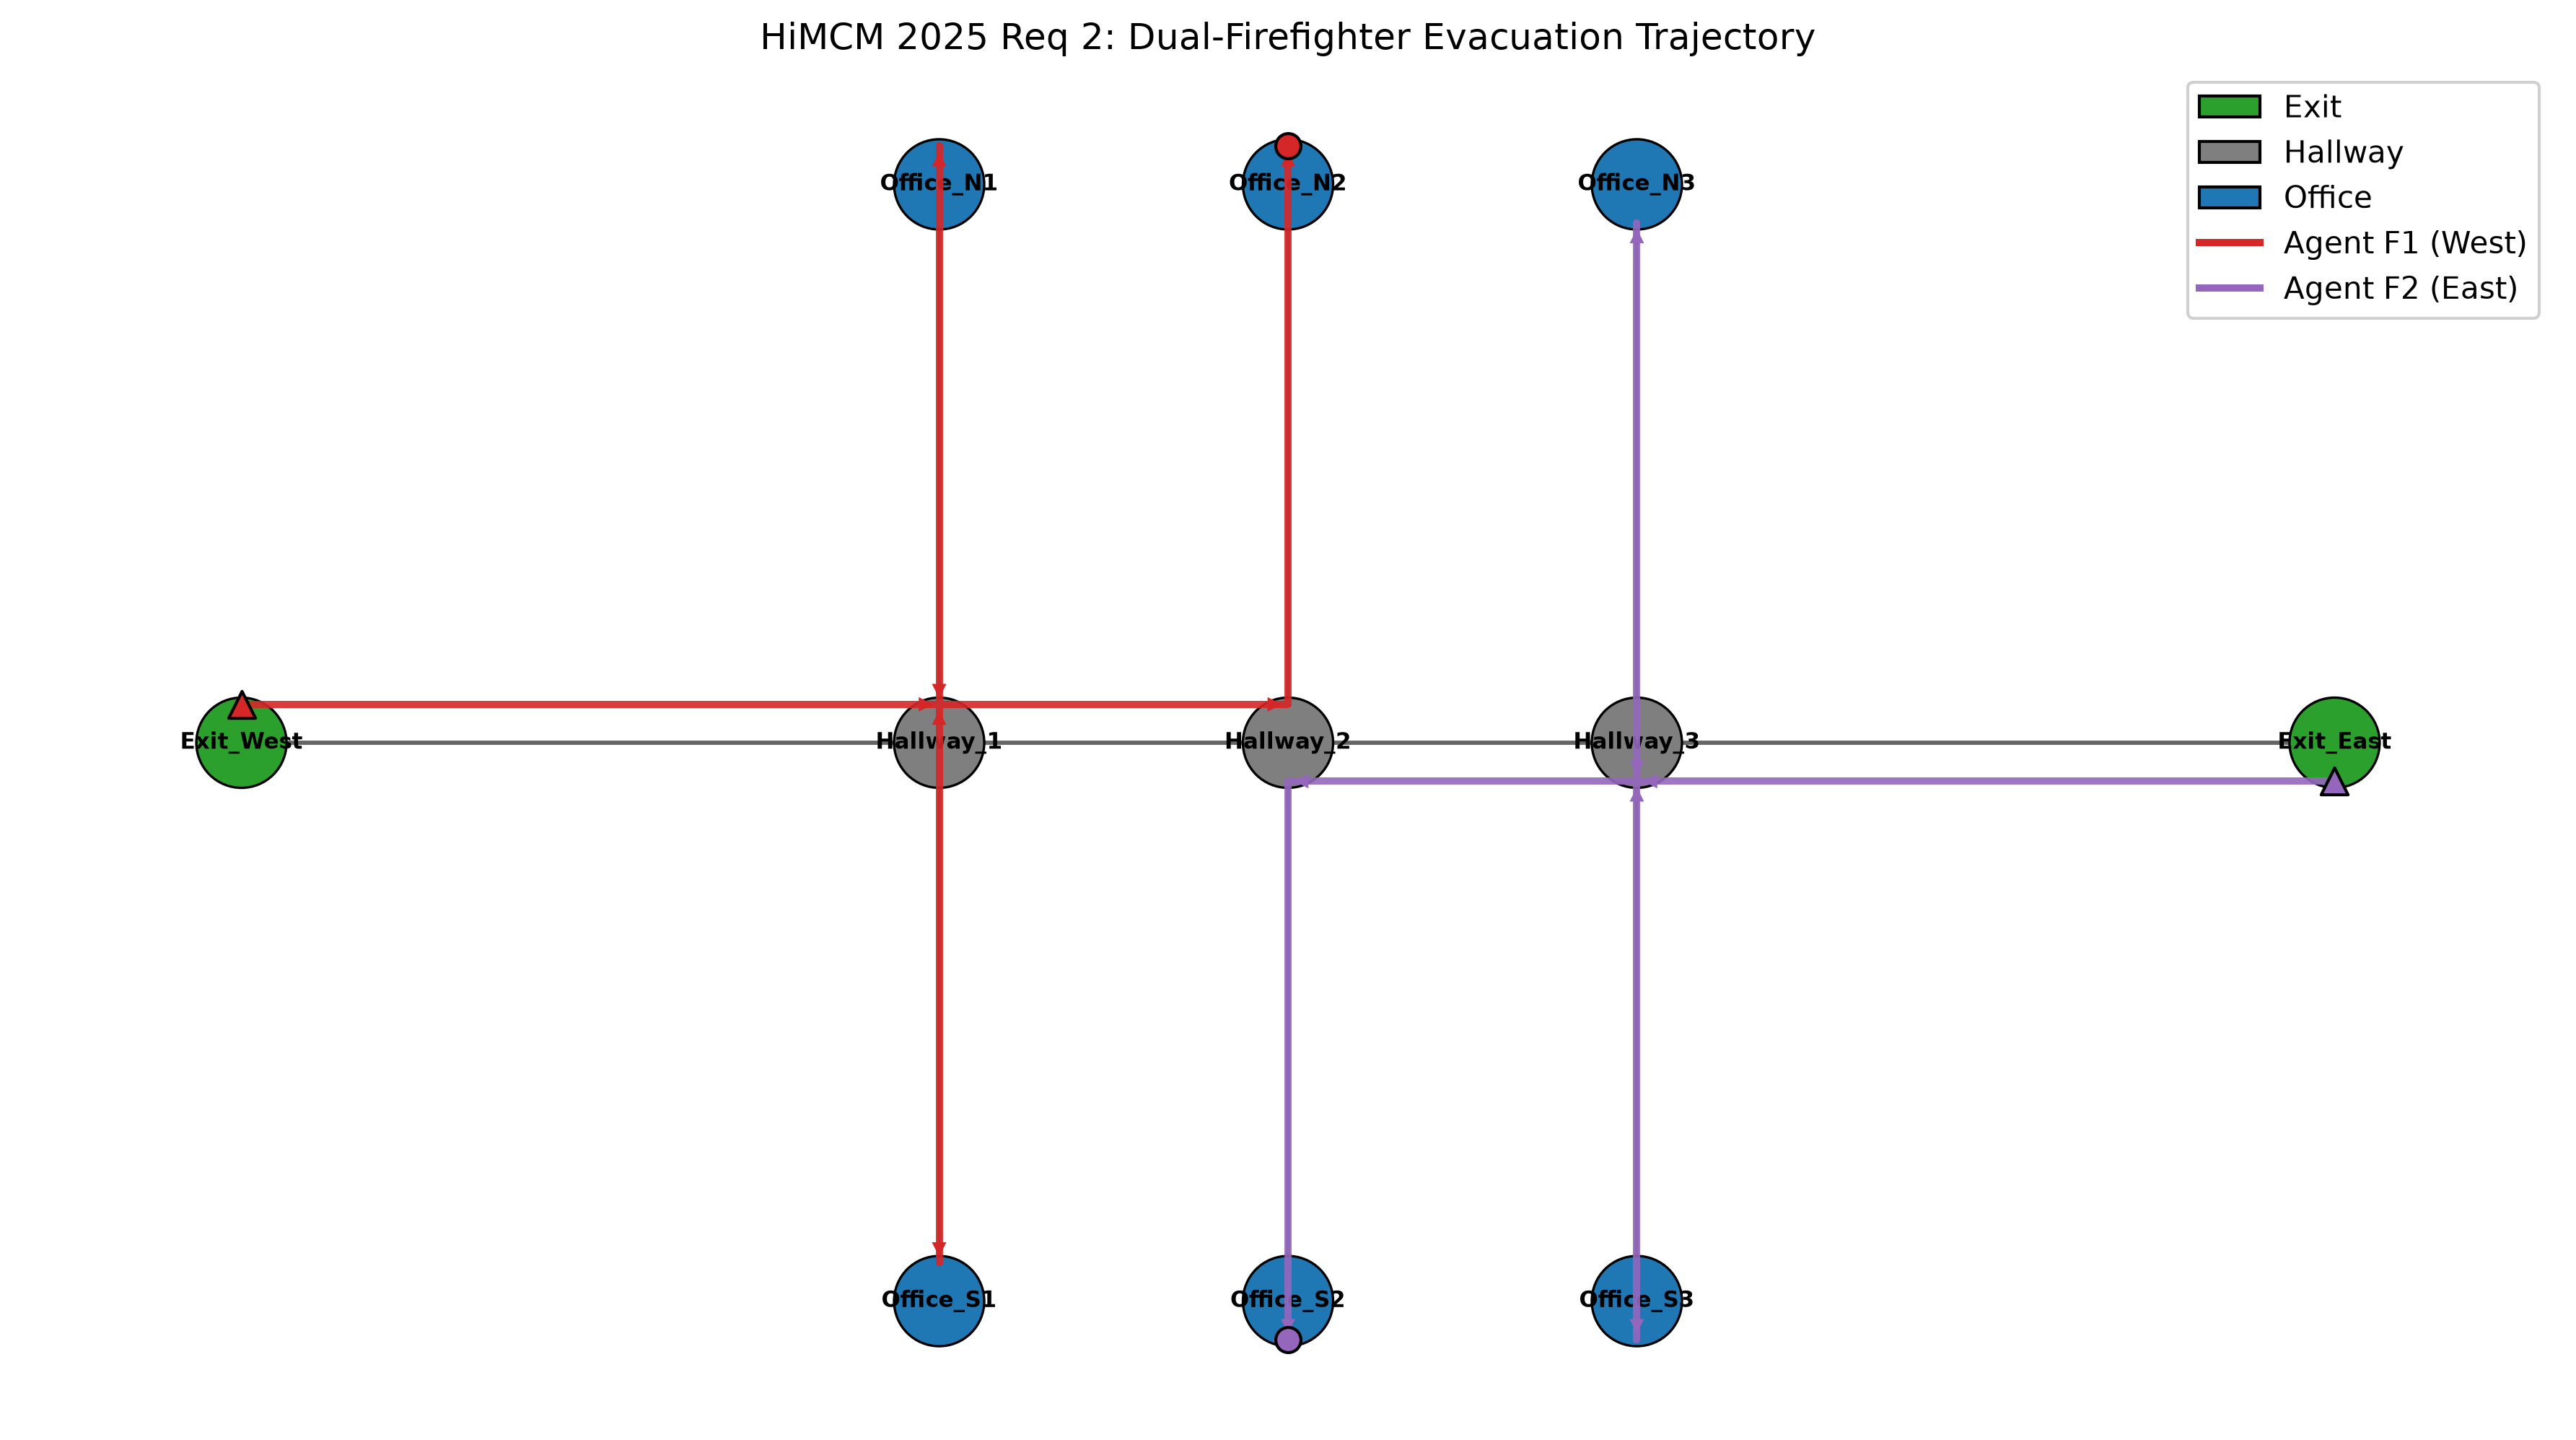
\includegraphics[width=0.92\textwidth]{office_sweep_trajectory.png}
  \caption{Figure~1 office: dual-firefighter trajectories produced by the scoring
  planner. \(F_1\) (west, red) clears \(N_1,S_1,N_2\); \(F_2\) (east, purple) clears
  \(N_3,S_3,S_2\). Repeated visits to a hallway hub are tree backtracks, not
  assignment oscillations.}
  \label{fig:office-traj}
\end{figure}

Monte Carlo confirmation under the ideal (no-smoke) condition, \(N=30\), is
deterministic: every replication reports \(\Tclear=135.0\,\mathrm{s}\),
\(\eta=1\), \(\rho=0\) (Table~\ref{tab:clear}).

%----------------------------------------------------------------------
\section{Scaled Multi-Agent Sweep Model (Daycare \& Warehouse Case Studies)}
\label{sec:req3}

\subsection{Scoring planner}

Idle firefighter \(a\) at node \(u\) scores each untagged room \(r\in R\) by
\begin{equation}
  \label{eq:score}
  \begin{aligned}
  \mathrm{Score}(r)
  &= -w_{\mathrm{dist}}\,d(u,r)
     -w_{\mathrm{hazard}}\,h(r)
     +w_{\mathrm{priority}}\,v(r)\\
  &\quad -w_{\mathrm{redundancy}}\mathbf{1}[r\text{ already targeted}]
     -w_{\mathrm{tabu}}\mathbf{1}[r\in T_a]
     +w_{\mathrm{mom}}M(a,r).
  \end{aligned}
\end{equation}
Here \(d(u,r)\) is shortest-path length (m) on the passable subgraph; \(h(r)\) is
smoke density plus a fire indicator; \(T_a\) is a tabu list of the last three
\emph{rooms} tagged by \(a\) (hallway cut-vertices are never forbidden); \(M(a,r)=1\)
if \(r\) shares a circulation hub with \(u\) (finish the column). Aspiration ignores
tabu when every remaining room is tabu. State machine:
\(\mathrm{move}\to\mathrm{sweep}\to\mathrm{tag}\to\mathrm{move}\).

Default weights:
\(w_{\mathrm{dist}}=1\), \(w_{\mathrm{hazard}}=8\) (experiments) or \(5\) (office demo),
\(w_{\mathrm{priority}}=2\), \(w_{\mathrm{redundancy}}=80\),
\(w_{\mathrm{tabu}}=50\), \(w_{\mathrm{mom}}=15\), tenure \(3\).

\subsection{Layouts}

\paragraph{Daycare.}
Three floors, six rooms per floor (same hanging template as Figure~1), west/east
stair flights of \(8\,\mathrm{m}\), ground exits \(E_W,E_E\). Eighteen searchable
nodes; infant and nap rooms carry \(v(r)\in\{4.5,5\}\).

\paragraph{Warehouse.}
An \(8\times 12\) four-connected grid of \(4\,\mathrm{m}\) cells, rack obstacles,
eight exits, 40 searchable bays. Extra firefighters spawn at remaining exits then
aisles.

\subsection{Ideal-condition results (Requirement~3)}

Table~\ref{tab:clear} reports mean \(\Tclear\) from 30 replications. The planner is
deterministic without fire, so the sample standard deviation is identically zero and
the 95\% Student-\(t\) interval collapses to a point---visible as zero-length error
bars in Figure~\ref{fig:personnel}.

\begin{table}[htbp]
\centering
\caption{Ideal (no-smoke) clearance. Source:
\texttt{results/experiment\_summary.csv}, \(N=30\).}
\label{tab:clear}
\begin{tabular}{@{}lrrrrr@{}}
\toprule
Scenario & Crew \(m\) & \(\Tclear\) (s) & \(\eta\) & \(\rho\) & Full clear \\
\midrule
Office     & 2 & 135.00 & 1.00 & 0.000 & \(30/30\) \\
Daycare    & 2 & 439.00 & 1.00 & 0.000 & \(30/30\) \\
Daycare    & 3 & 300.67 & 1.00 & 0.000 & \(30/30\) \\
Daycare    & 4 & 255.67 & 1.00 & 0.111 & \(30/30\) \\
Warehouse  & 3 & 424.67 & 1.00 & 0.700 & \(30/30\) \\
Warehouse  & 4 & 333.00 & 1.00 & 0.750 & \(30/30\) \\
Warehouse  & 5 & 262.33 & 1.00 & 0.775 & \(30/30\) \\
\bottomrule
\end{tabular}
\end{table}

\begin{figure}[htbp]
  \centering
  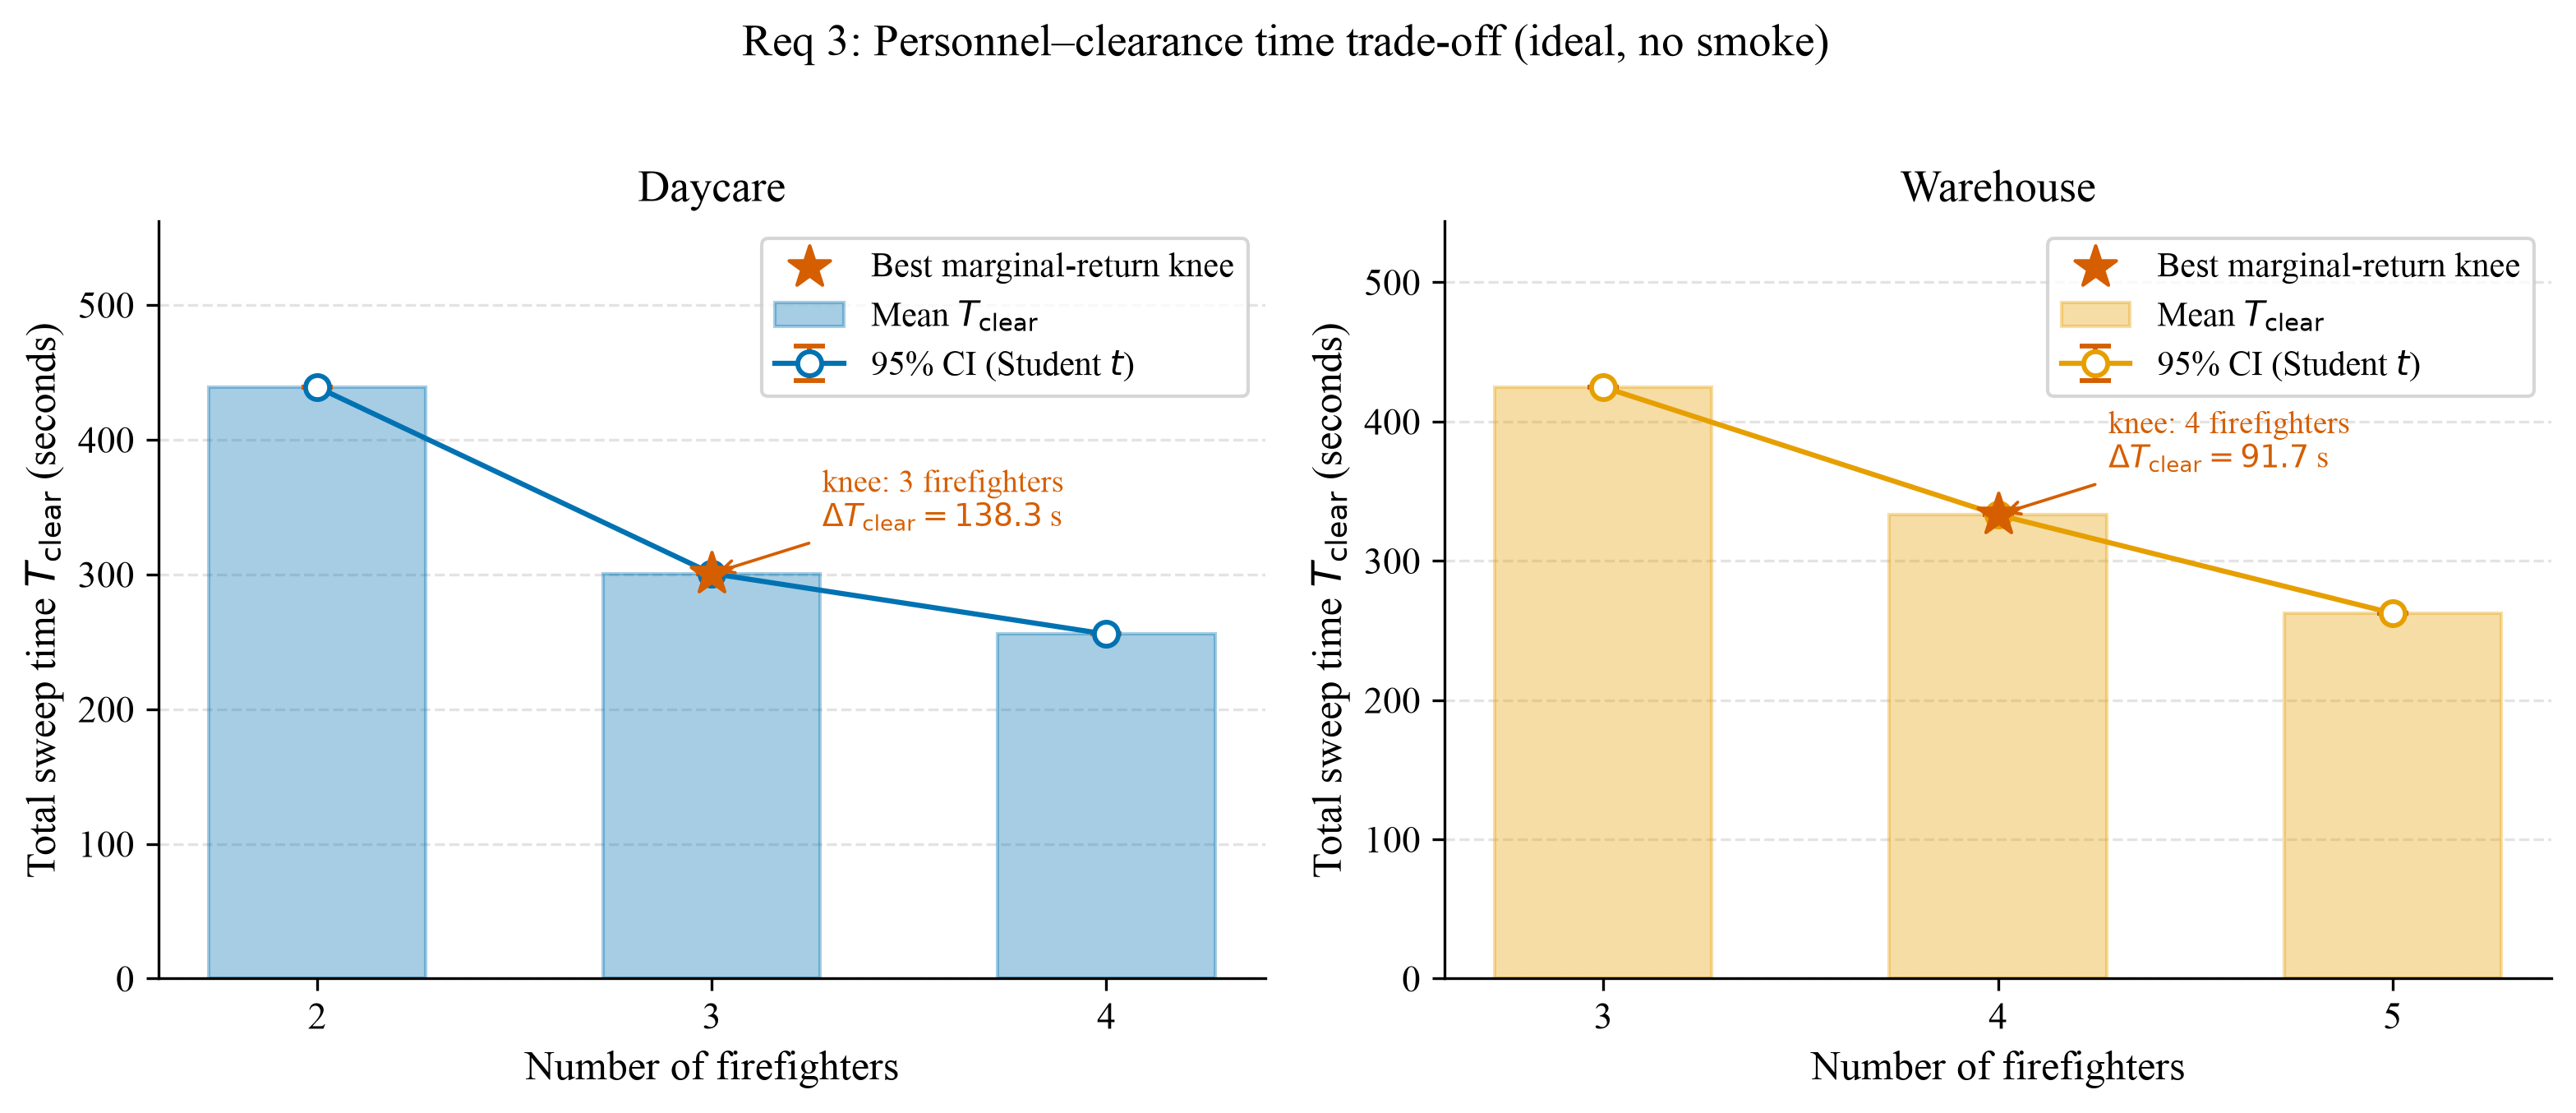
\includegraphics[width=0.98\textwidth]{fig1_personnel_tradeoff.png}
  \caption{Requirement~3 personnel--time trade-off under the ideal condition.
  Stars mark the crew size that realises the largest one-firefighter reduction
  \(\Delta\Tclear=\Tclear(m-1)-\Tclear(m)\): daycare \(m=3\) (\(138.3\,\mathrm{s}\)),
  warehouse \(m=4\) (\(91.7\,\mathrm{s}\)).}
  \label{fig:personnel}
\end{figure}

\begin{figure}[htbp]
  \centering
  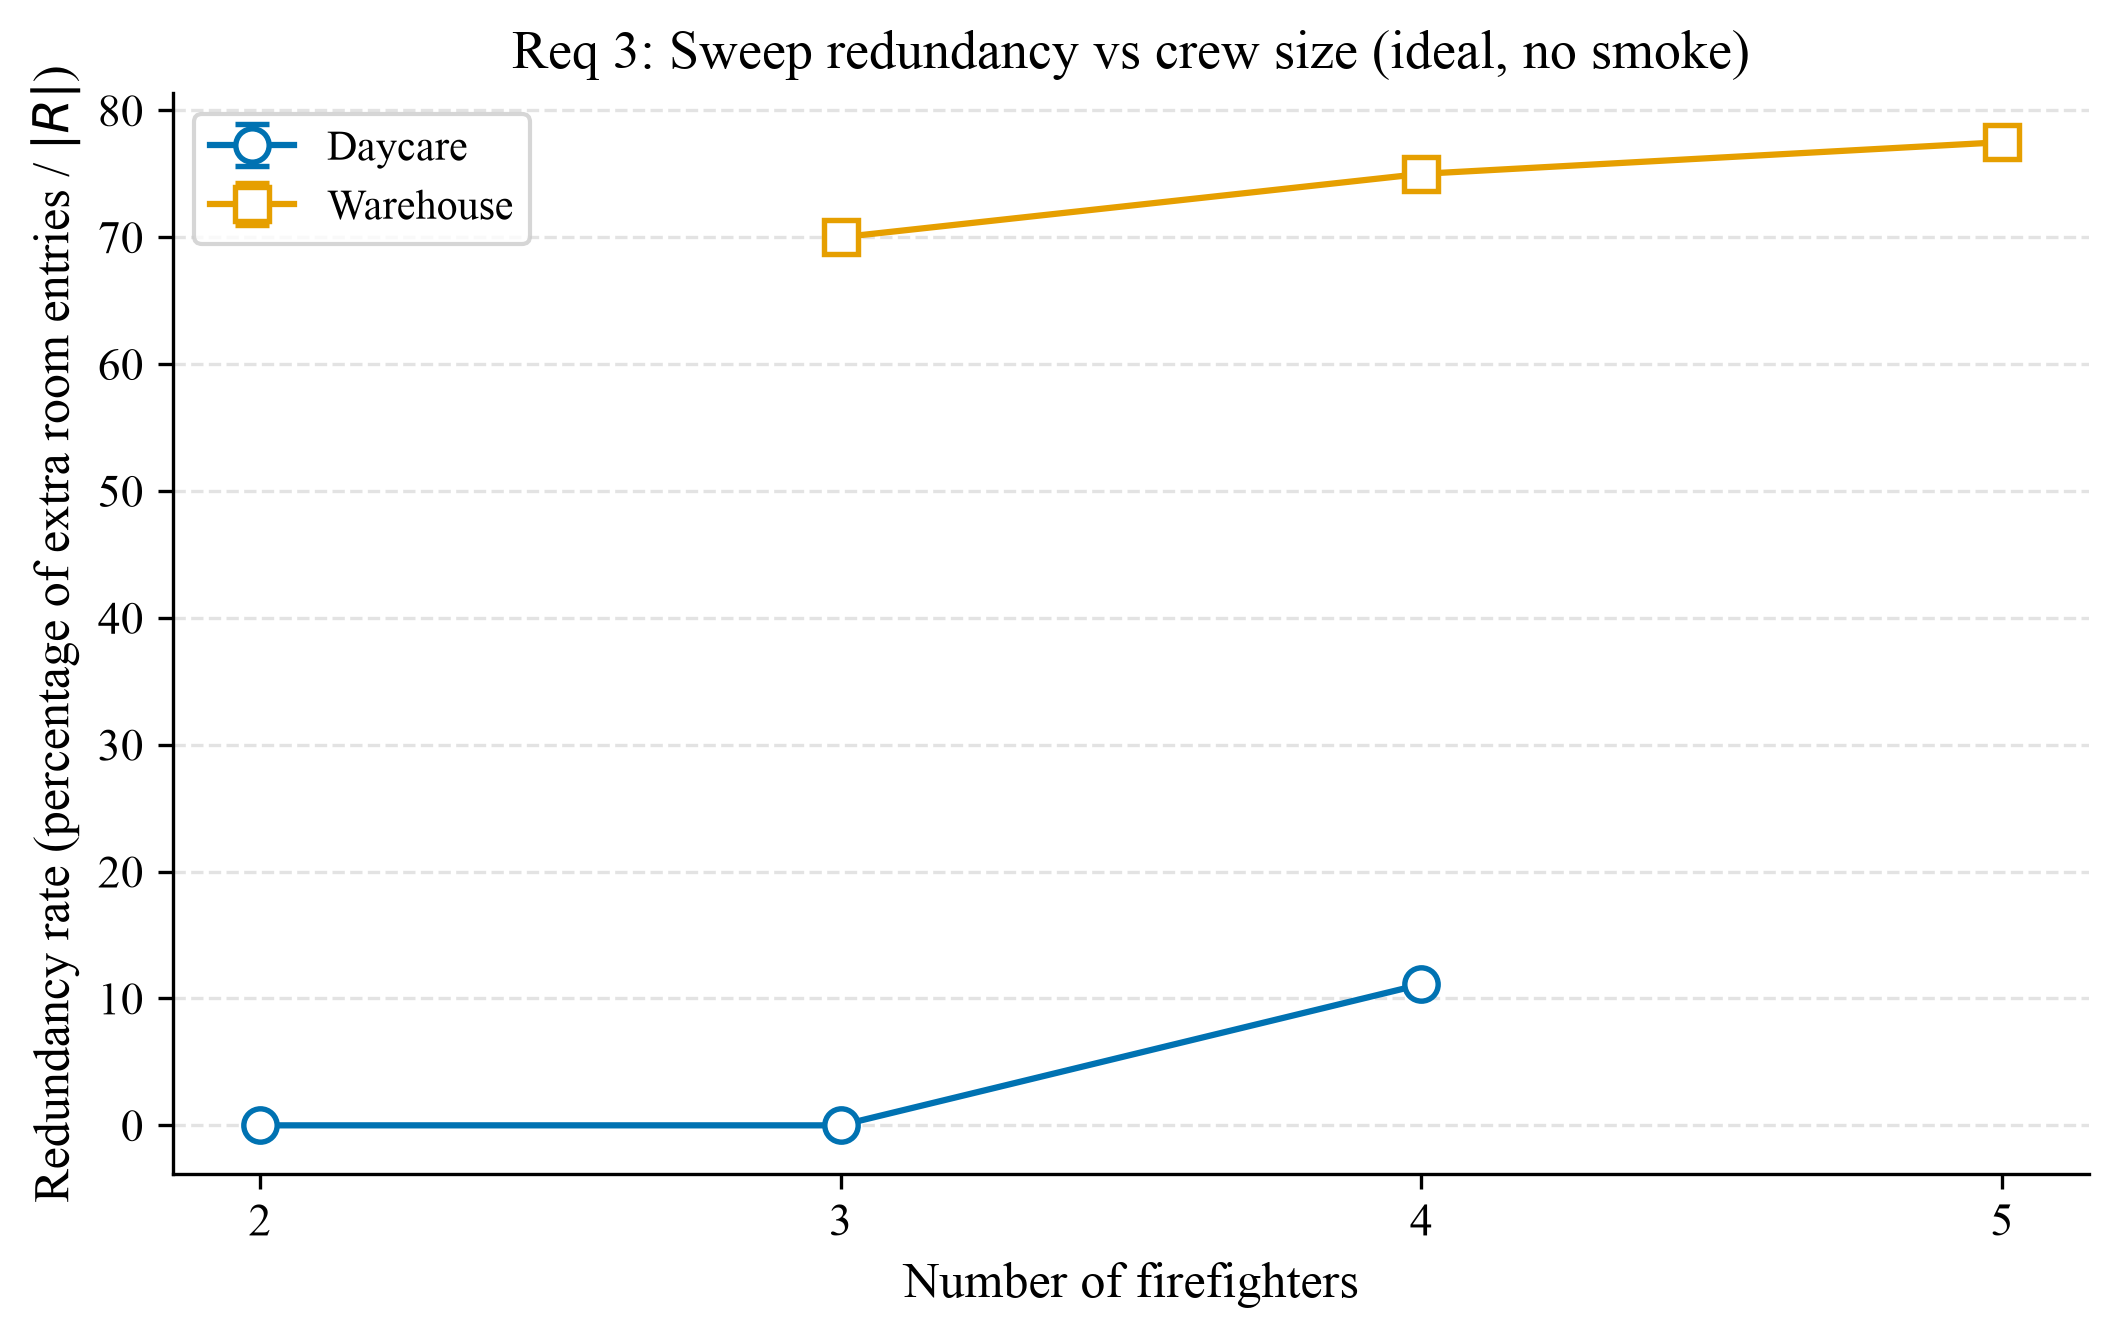
\includegraphics[width=0.78\textwidth]{fig3_redundancy_tradeoff.png}
  \caption{Sweep redundancy \(\rho\) (percent extra searchable entries per \(|R|\))
  versus crew size, ideal condition. Tree-like daycares stay near zero until the
  fourth firefighter; the warehouse grid induces \(70\)--\(78\%\) extra bay
  entries as more agents share aisles.}
  \label{fig:redundancy}
\end{figure}

\paragraph{Recommendation (no hazard).}
Send \textbf{three} firefighters to the daycare template and \textbf{four} to the
warehouse template if the objective is elapsed sweep time per additional person.
A fourth daycare firefighter still helps (\(-45\,\mathrm{s}\)) but is the first
crew size at which \(\rho\) becomes positive (\(0.111\)).

\subsection{GAT-PPO on the Figure~1 office}
\label{sec:gat-ppo}

The scoring planner is a kinematic FSM: travel uses \(\whall\) and \(\vroom\),
and a room tag costs \(\tsw+\ttag=25\,\mathrm{s}\) after the access edge.
GAT-PPO instead acts on the unweighted office graph. Each agent, at every
discrete graph step, either stays (the stay action is the only way to tag the
current searchable node) or walks one incident edge. Team reward is
\begin{equation}
  \label{eq:rl-reward}
  R
  = 10\,\Delta |R_{\mathrm{tagged}}|
    -0.5
    -2\,\mathbf{1}_{\mathrm{redundant}}
    +50\,\mathbf{1}_{\mathrm{all\,clear}},
\end{equation}
with an additional \(-15\) if a firefighter occupies a burning node (disabled in
the office pre-train). The actor-critic is a two-layer GAT (\(4\) heads,
hidden width \(64\), residual LayerNorm) with masked softmax over
\(1+\deg(u)\) actions and attentional critic pooling. We train parameter-shared
PPO for \(200\) episodes, \(\gamma=0.99\), GAE \(\lambda=0.95\), clip \(0.2\),
entropy bonus \(0.01\), two agents, no fire
(\texttt{src/rl/checkpoints/gat\_ppo\_office.pt}).

Because one graph step is not one second, we compare \emph{full-clearance rate}
and \emph{rooms tagged}, not \(\Tclear\) in seconds. Evaluation uses the same
checkpoint with two decoding modes, \(N=30\) each, episode seeds \(1000{+}i\)
(greedy) and \(2000{+}i\) (stochastic), and a matching Torch RNG seed so the
CSV is reproducible (Table~\ref{tab:rl},
\texttt{results/rl\_office\_eval.csv}).

\begin{table}[htbp]
\centering
\caption{Office \(m=2\), ideal (no smoke). Planner row from
\texttt{experiment\_summary.csv}; GAT-PPO from
\texttt{rl\_office\_eval.csv}, \(N=30\). Rooms and steps for GAT-PPO are
sample means with 95\% \(t\) intervals. Planner steps are kinematic seconds,
not graph hops.}
\label{tab:rl}
\begin{tabular}{@{}lcccc@{}}
\toprule
Policy & Full clear & Rooms tagged & Length & Return \\
\midrule
Scoring planner & \(30/30\) & \(6.00\) & \(135\,\mathrm{s}\) & --- \\
GAT-PPO greedy & \(0/30\) & \(2.00\) & \(80.0\) hops & \(-172.0\) \\
GAT-PPO stochastic & \(20/30\) & \(5.60\ [5.37,5.83]\) &
  \(59.3\ [52.2,66.5]\) hops & \(18.7\ [-2.4,39.9]\) \\
\bottomrule
\end{tabular}
\end{table}

Greedy \(\mathrm{argmax}\) decoding collapses: every trial hits the
\(80\)-step cap with exactly two rooms tagged and return \(-172\). The trained
categorical still places mass on exploratory hops; sampling that distribution
fully clears \(20/30\) trials and tags \(5.60\) rooms on average
(Figure~\ref{fig:rl-vs-base}). Among successful stochastic rollouts, the
shortest recorded full clear in this evaluation used seed \(2014\) and
\(29\) graph steps (Figure~\ref{fig:rl-traj}). Boxplots of length and return
(Figure~\ref{fig:rl-eval}) show that stochastic decoding both shortens the
typical episode relative to the greedy timeout and yields a return whose
\(95\%\) interval still covers zero---the policy is useful but not a
substitute for the \(135\,\mathrm{s}\) FSM on this small tree.

\begin{figure}[htbp]
  \centering
  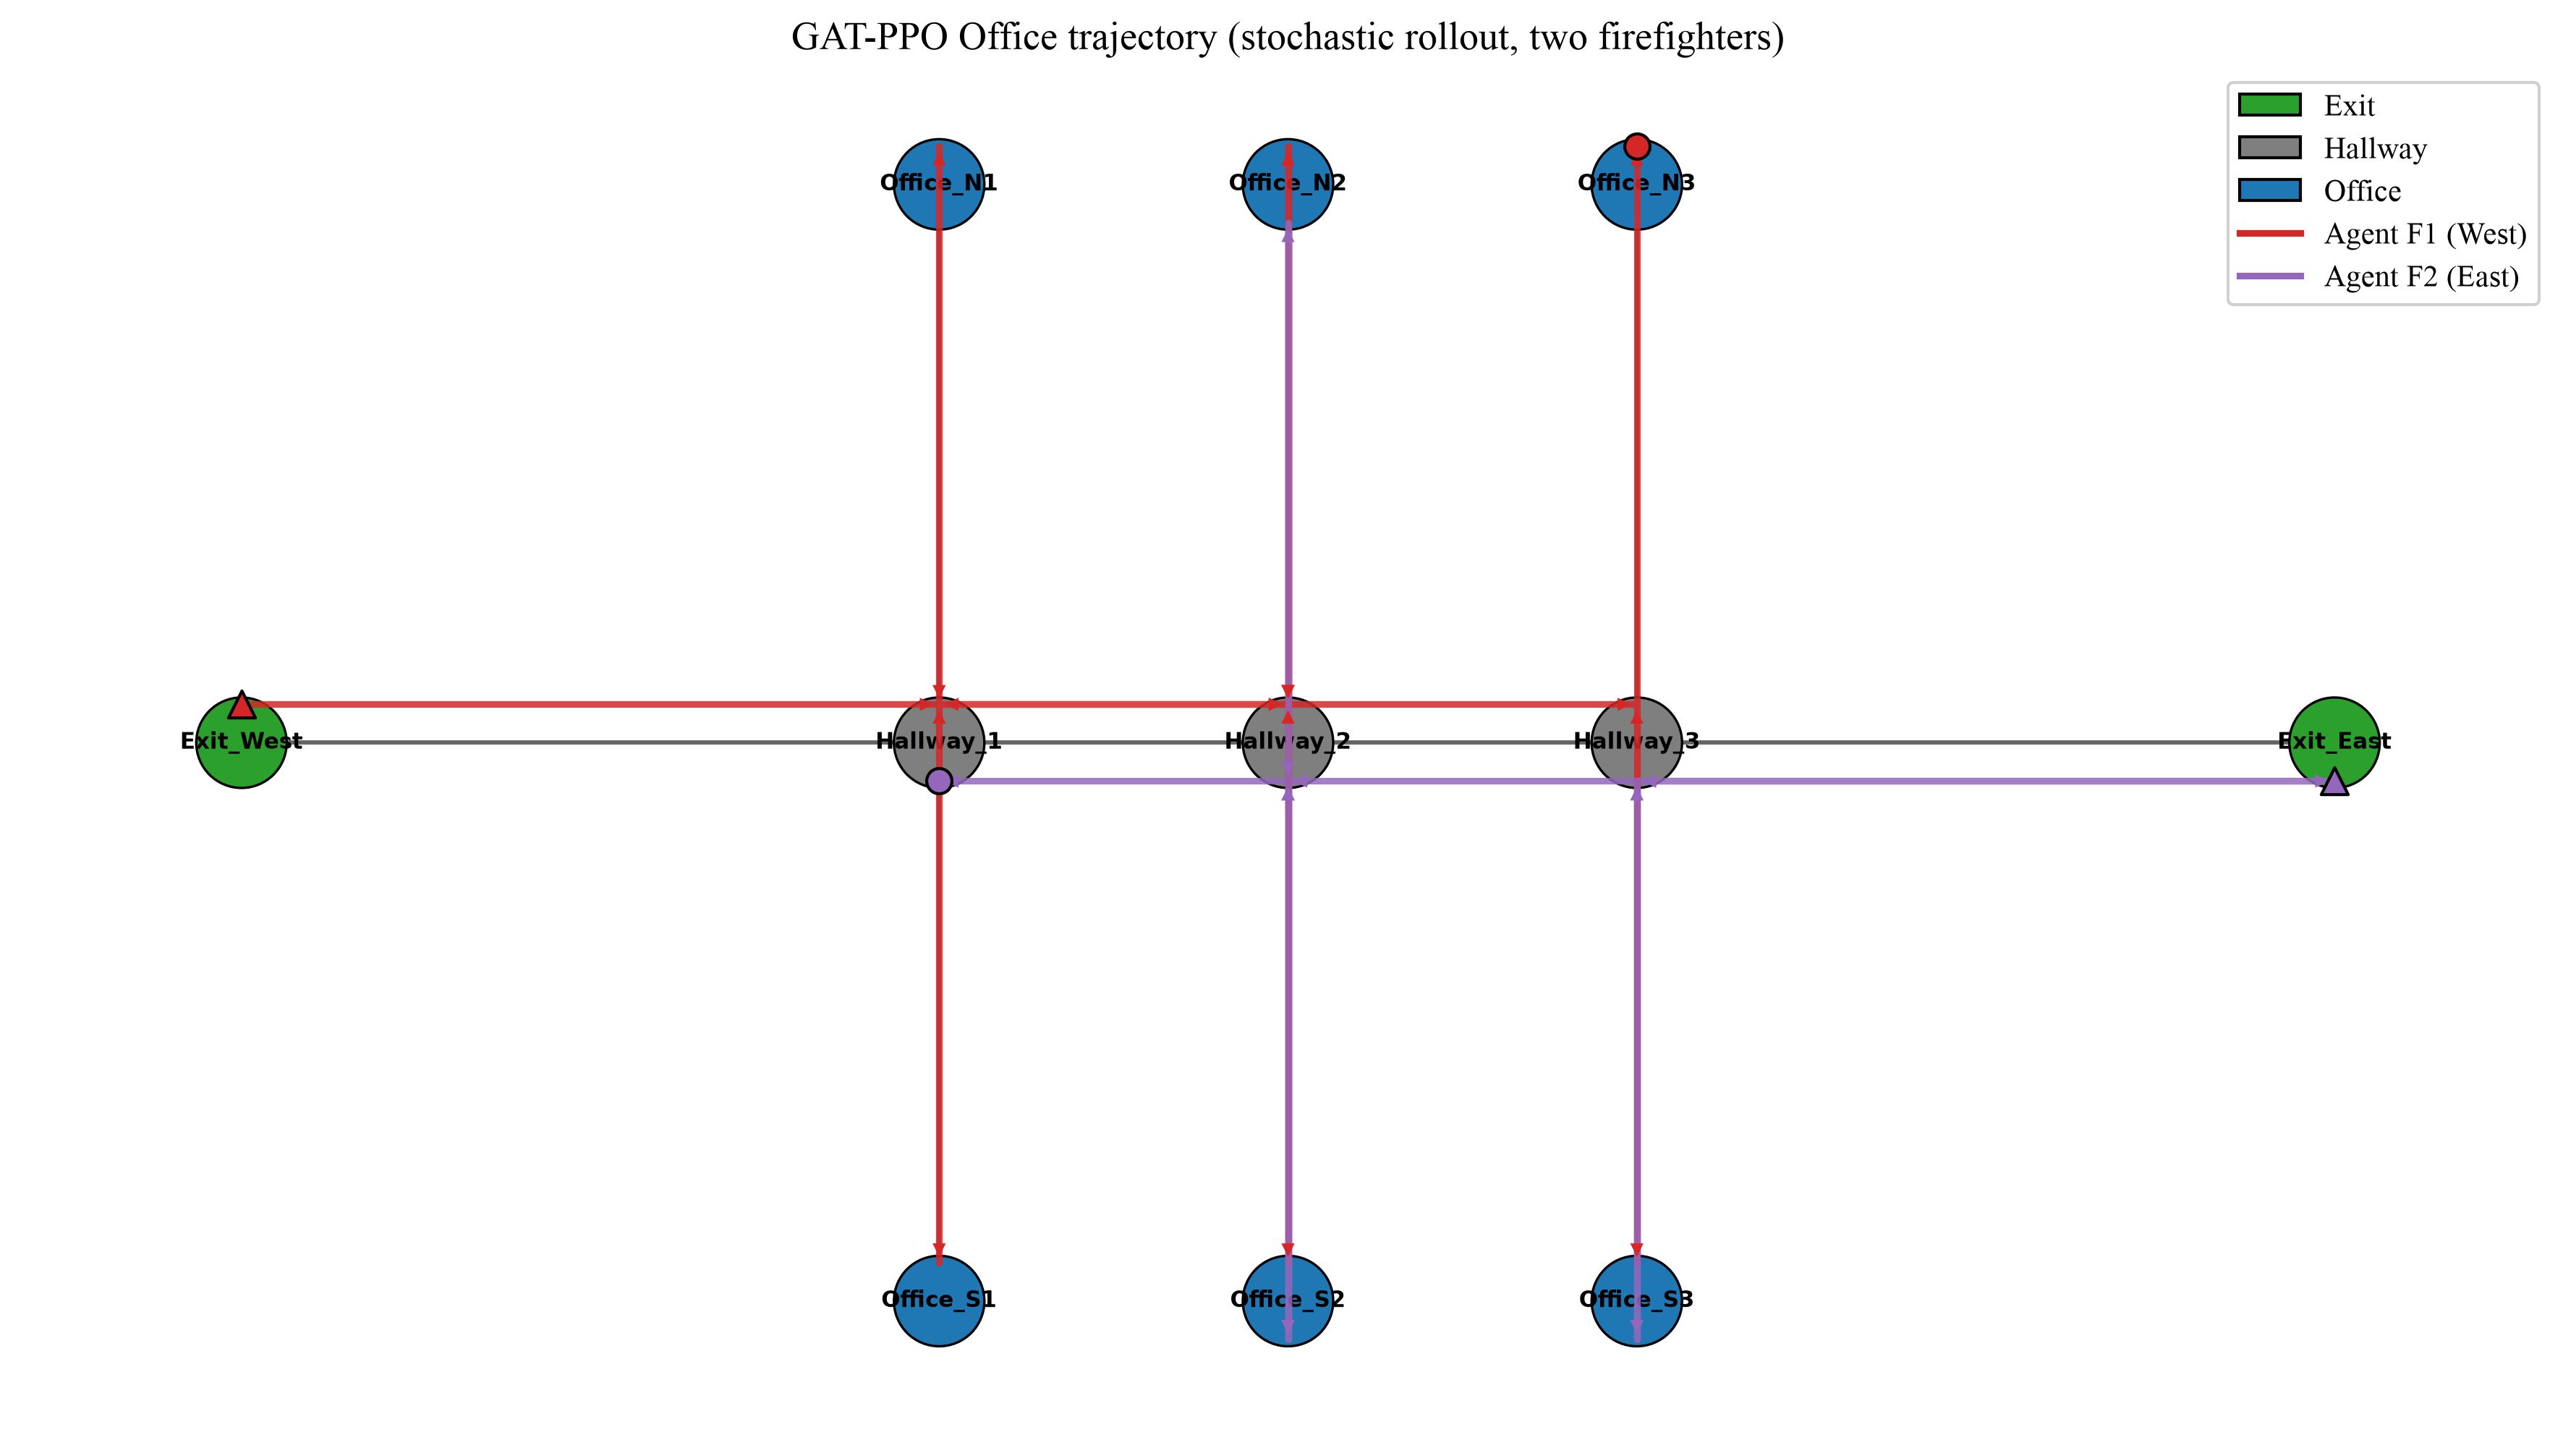
\includegraphics[width=0.92\textwidth]{fig4_rl_office_trajectory.png}
  \caption{GAT-PPO stochastic rollout on Figure~1 (seed \(2014\)): both agents
  start at the west/east exits (triangles) and finish at the marked discs after
  tagging all six offices in \(29\) graph steps. Stay actions appear as
  overlapping vertices rather than hallway backtracks.}
  \label{fig:rl-traj}
\end{figure}

\begin{figure}[htbp]
  \centering
  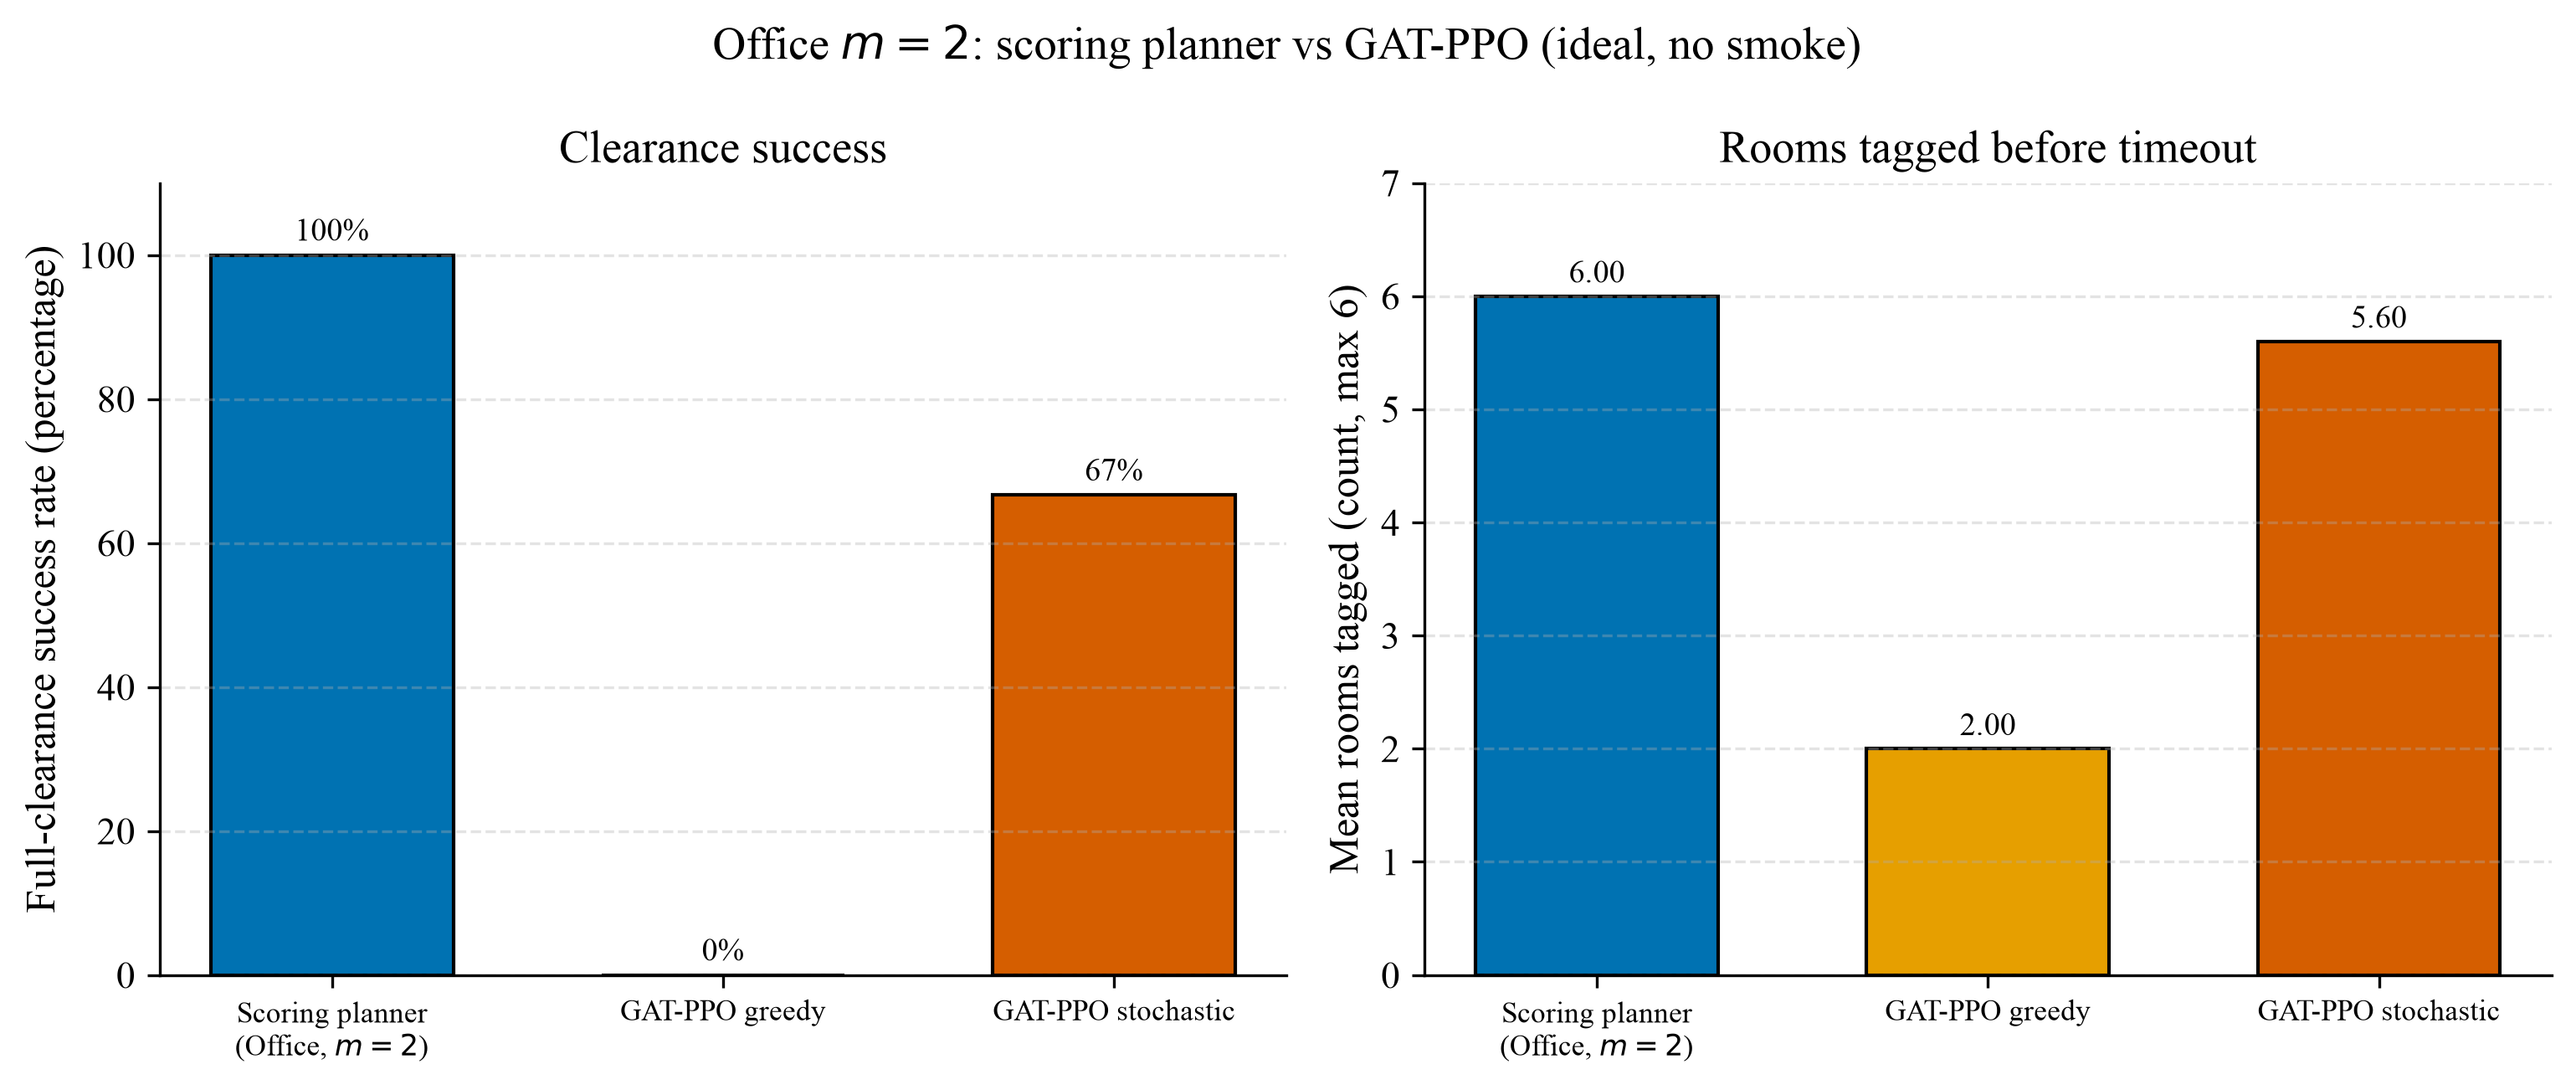
\includegraphics[width=0.98\textwidth]{fig5_baseline_vs_rl.png}
  \caption{Office \(m=2\), ideal condition: full-clearance rate and mean rooms
  tagged. The scoring planner is \(30/30\) and \(6/6\). GAT-PPO greedy is
  \(0/30\); stochastic decoding is \(20/30\) with mean \(5.60\) rooms.
  Source: \texttt{experiment\_summary.csv} and \texttt{rl\_office\_eval.csv}.}
  \label{fig:rl-vs-base}
\end{figure}

\begin{figure}[htbp]
  \centering
  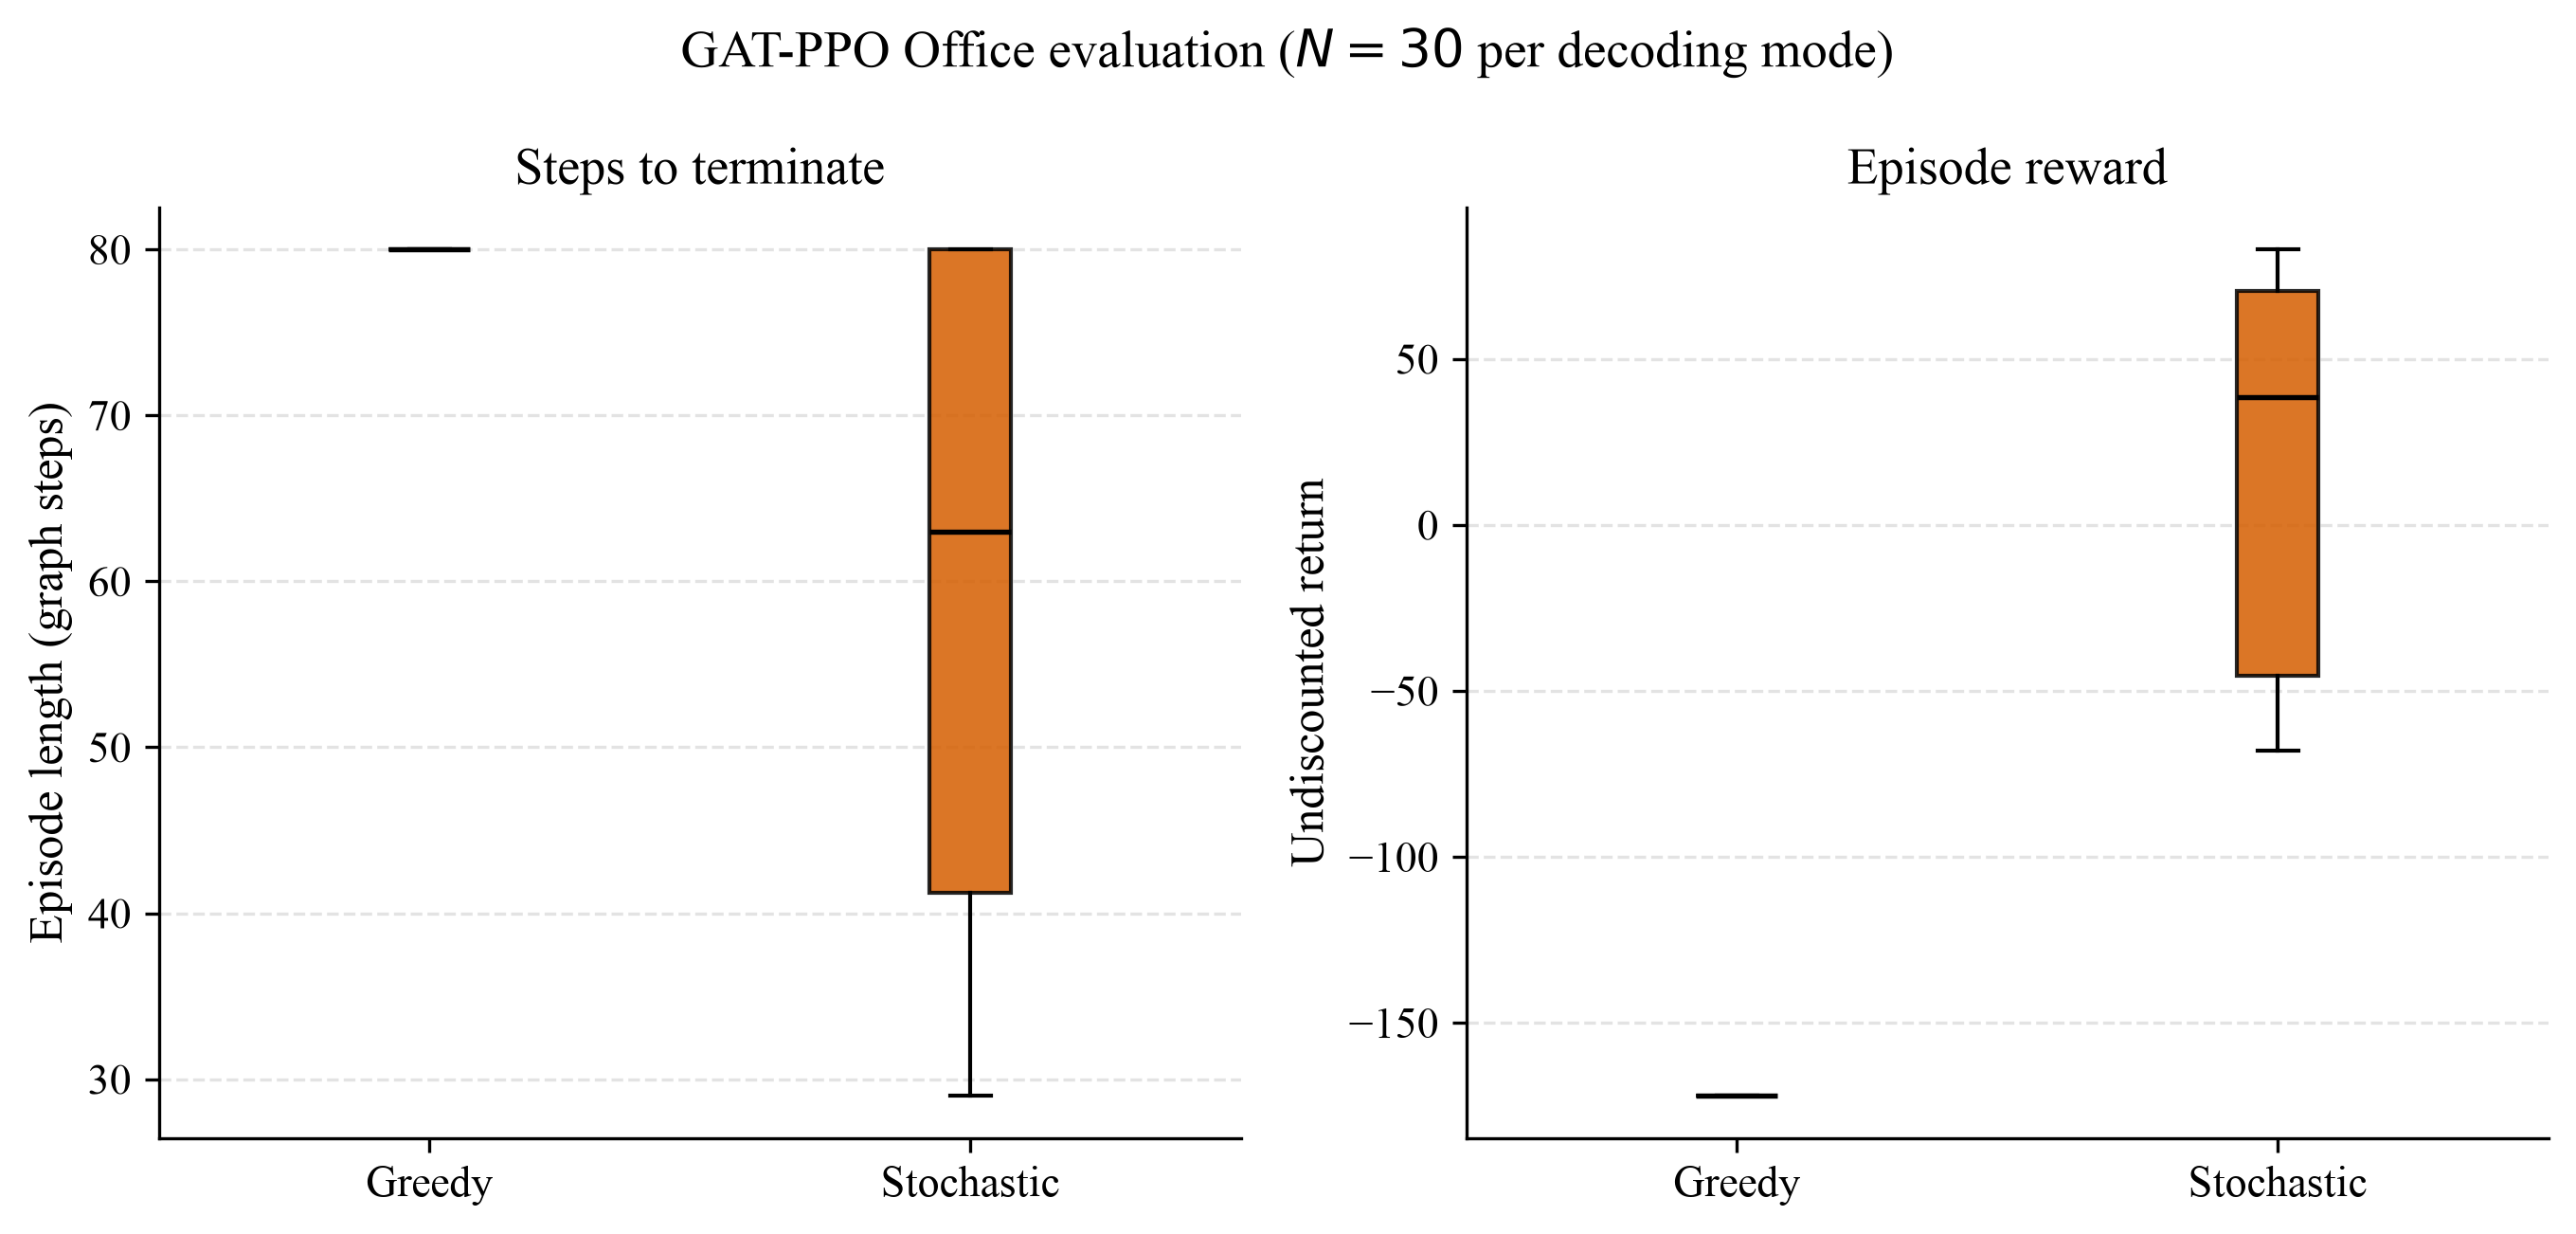
\includegraphics[width=0.88\textwidth]{fig6_rl_policy_eval.png}
  \caption{GAT-PPO Office evaluation, \(N=30\) per decoding mode. Greedy
  decoding is degenerate (exactly \(80\) hops, return \(-172\)). Stochastic
  decoding has mean length \(59.3\) hops and mean return \(18.7\).}
  \label{fig:rl-eval}
\end{figure}

\paragraph{Recommendation (learned policy).}
Use the scoring planner for contest-ready \(\Tclear\) in seconds. Use
stochastic GAT-PPO only as a graph covering prior: it can finish the six-room
office in a majority of sampled trials, but greedy inference is currently
unsafe (stay bias), and the hop clock is not a fireground timeline.

%----------------------------------------------------------------------
\section{Real-World Hazards \& Sensor Technology Integration}
\label{sec:req4}

\subsection{Fire and smoke on the graph}

Let \(k(u)\) be the number of burning neighbours of \(u\). Ignition of a cold node
in one discrete hazard step occurs with
\begin{equation}
  \label{eq:pspread}
  P_{\mathrm{spread}}(u)
  = 1-(1-p_0)^{k(u)}, \qquad p_0=0.08
\end{equation}
in the Monte Carlo engine. Smoke advances by a multi-source Dijkstra cutoff of
length \(v_{\mathrm{smoke}}\Delta t\) with
\(v_{\mathrm{smoke}}=1.5\,v_{\mathrm{fire}}\) and \(v_{\mathrm{fire}}=0.45\,\mathrm{m/s}\).
Density \(\sigma(u)\in[0,1]\) yields speed multiplier
\(\max(0.15,1-0.4\sigma(u))\) and visibility
\(\max(0.10,1-0.8\sigma(u))\). Fully involved nodes are impassable.

Each smoke trial draws a uniform ignition node from rooms, bays, and hallways
(exits excluded) and a distinct RNG seed
\(2025+10^{5}s+10^{3}m+100\cdot\mathbf{1}_{\mathrm{smoke}}+\mathrm{run\_id}\).

\subsection{What the 210 smoke trials actually show}

Full-building clearance success was \(0/210\). On the small office and daycare
graphs, fire cuts the unique hallway spine; agents deadlock after tagging only a
few rooms. Warehouse trials last longer (median abort \(\approx 182\)--\(192\,\mathrm{s}\))
and salvage more bays, but five runs hit the 5000-step cap (\(\Tclear\) recorded as
\(10\,000\,\mathrm{s}\)). Those abort clocks are \emph{not} sweep times; we therefore
report salvage \(\eta\) and median abort time, not mean \(\Tclear\), for smoke
(Table~\ref{tab:smoke}).

\begin{table}[htbp]
\centering
\caption{Dynamic smoke (\(p_0=0.08\)). Salvage \(\eta\) is a 95\% \(t\)-interval
over \(N=30\). Median abort time excludes the interpretation of timeouts as
completed sweeps. Source: \texttt{experiment\_summary.csv}.}
\label{tab:smoke}
\begin{tabular}{@{}lrrcccc@{}}
\toprule
Scenario & \(m\) & Full clear & \(\eta\) mean [95\% CI] & Med.\ abort (s) & Med.\ rooms tagged \\
\midrule
Office    & 2 & \(0/30\) & \(0.200\ [0.130,0.270]\) & 42.0 & 1 \\
Daycare   & 2 & \(0/30\) & \(0.158\ [0.130,0.186]\) & 50.5 & 2 \\
Daycare   & 3 & \(0/30\) & \(0.197\ [0.169,0.225]\) & 46.0 & 3 \\
Daycare   & 4 & \(0/30\) & \(0.267\ [0.241,0.293]\) & 56.5 & 4 \\
Warehouse & 3 & \(0/30\) & \(0.322\ [0.285,0.358]\) & 182.0 & 12.5 \\
Warehouse & 4 & \(0/30\) & \(0.403\ [0.363,0.444]\) & 182.0 & 15.0 \\
Warehouse & 5 & \(0/30\) & \(0.532\ [0.476,0.589]\) & 192.0 & 21.5 \\
\bottomrule
\end{tabular}
\end{table}

\begin{figure}[htbp]
  \centering
  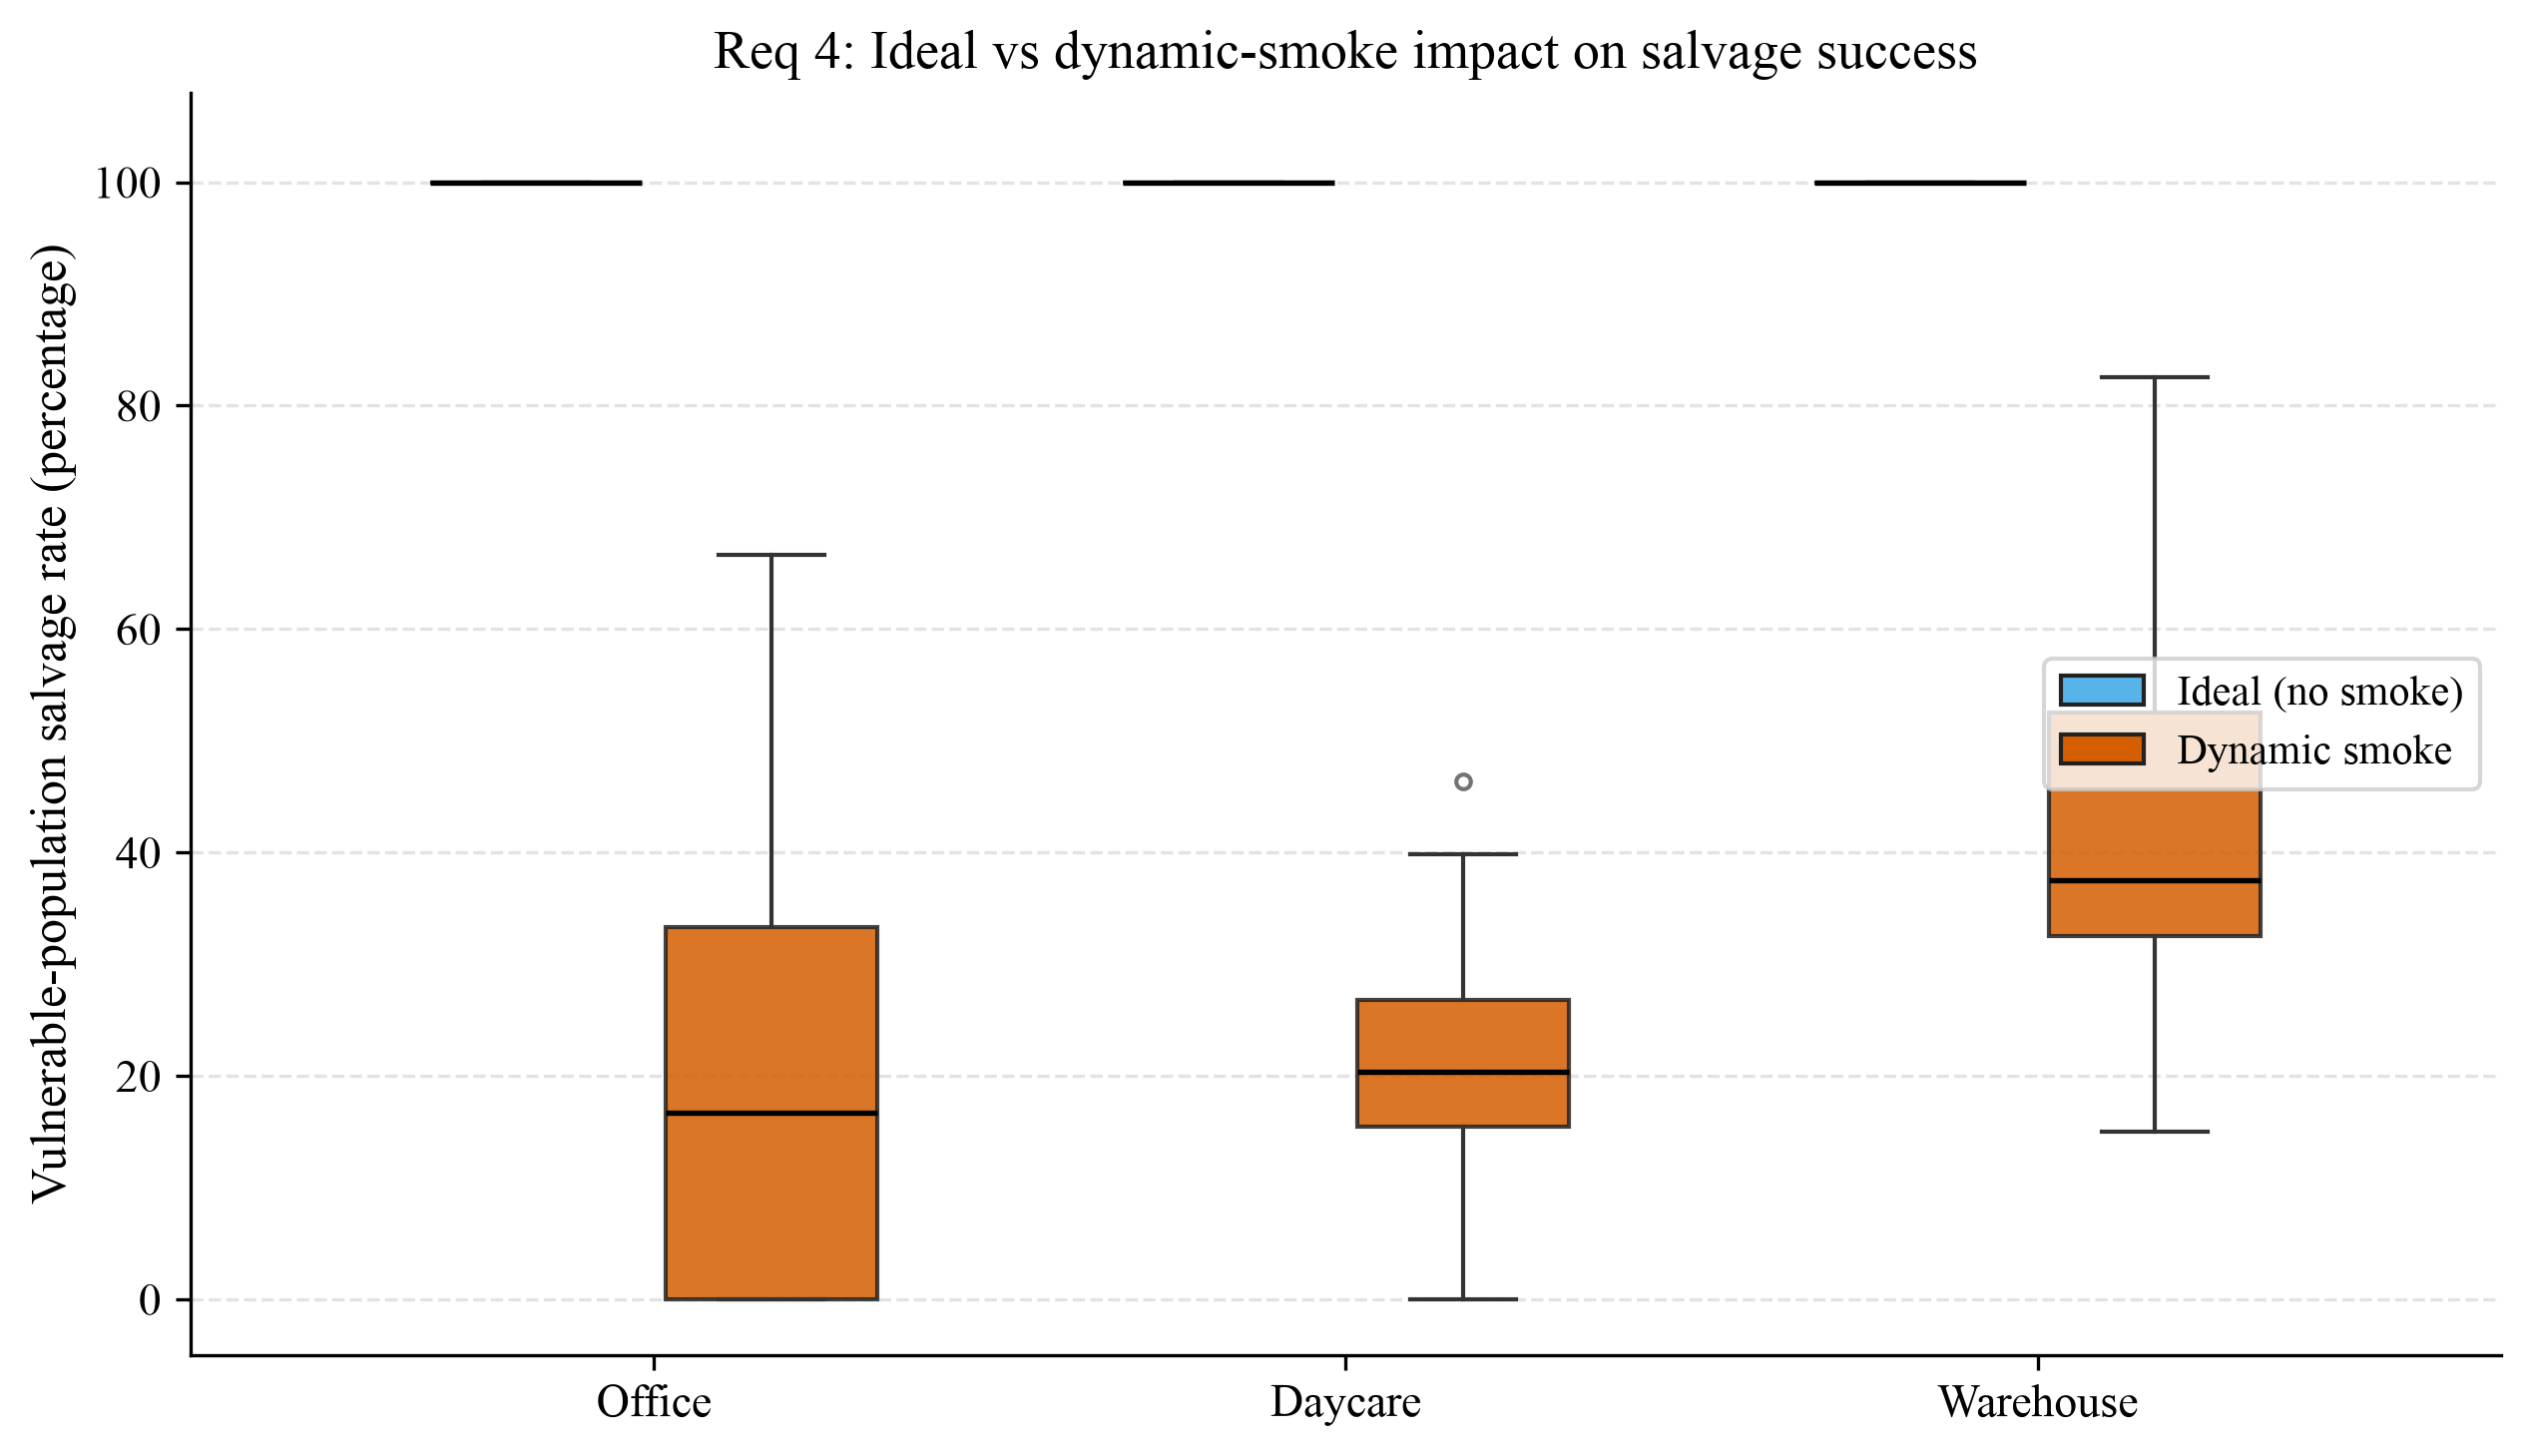
\includegraphics[width=0.88\textwidth]{fig2_hazard_impact.png}
  \caption{Requirement~4: distribution of vulnerable-population salvage \(\eta\)
  (percentage) under ideal versus dynamic-smoke conditions, pooling crew sizes
  within each building. Ideal mass sits at \(100\%\); smoke mass is strictly
  below, with the warehouse retaining the highest median salvage.}
  \label{fig:hazard}
\end{figure}

Crew size still has a monotone effect \emph{inside} the hazard: daycare salvage
rises \(15.8\%\to 19.7\%\to 26.7\%\) for \(m=2,3,4\); warehouse
\(32.2\%\to 40.3\%\to 53.2\%\) for \(m=3,4,5\). Extra agents tag more high-\(v(r)\)
rooms before the graph disconnects; they do not restore full clearance at this
\(p_0\).

\subsection{Sensor technology as model inputs}

We do not simulate proprietary hardware. We specify how three sensor classes would
enter~\eqref{eq:score} without changing the planner API.
\begin{itemize}[leftmargin=1.2em]
  \item \textbf{Door tags / NFC ``cleared'' cards.}
        Already modelled as \(\ttag=5\,\mathrm{s}\). A digital tag that broadcasts
        to all radios sets the shared tagged-set instantly, which is our current
        information assumption.
  \item \textbf{Thermal or through-smoke cameras.}
        Reduce \(\tsw\) and raise visibility; equivalently increase \(M(a,r)\) for
        rooms already viewed from the hallway, or lower \(h(r)\) when the camera
        reports a cold empty volume.
  \item \textbf{Heat/CO detectors and helmet-mounted lidar.}
        Provide an estimate of \(k(u)\) and \(\sigma(u)\) ahead of physical arrival,
        which is exactly the field \(h(r)\) already subtracted in~\eqref{eq:score}.
        A more conservative \(w_{\mathrm{hazard}}\) is then a policy choice, not a
        new algorithm.
\end{itemize}
The Monte Carlo says that without such lookahead, \(p_0=0.08\) on a single-spine
building is operationally unsurvivable as a \emph{full} primary search. Sensors
matter because they either slow effective spread (earlier isolation) or let agents
skip already-scanned volumes.

%----------------------------------------------------------------------
\section{Sensitivity \& Robustness Analysis}
\label{sec:req5}

\subsection{Crew size (ideal)}

Figure~\ref{fig:personnel} is the principal sensitivity of \(\Tclear\) to \(m\).
Marginal returns diminish: daycare savings \(138.3\,\mathrm{s}\) then
\(45.0\,\mathrm{s}\); warehouse \(91.7\,\mathrm{s}\) then \(70.7\,\mathrm{s}\).
The recommendation in Section~\ref{sec:req3} is this discrete derivative, not a
continuous EOQ formula.

\subsection{Hazard on/off}

Switching from \texttt{clear} to \texttt{smoke} is a binary stress test. Full-clearance
rate drops from \(1\) to \(0\) in every building at \(p_0=0.08\). The robust
\emph{ranking} of buildings by salvage under smoke is warehouse \(>\) daycare
\(\approx\) office, consistent with extra exits and grid connectivity. \(\eta\)
intervals in Table~\ref{tab:smoke} do not overlap the ideal value \(1\), so the
hazard effect is not a sampling artefact.

\subsection{Determinism and confidence intervals}

With fire off, 30 seeds produce bit-identical \(\Tclear\). Reporting a 95\% CI
is then a formality (width \(0\)). With fire on, \(\eta\) has genuine dispersion
driven by the random ignition node; office salvage 95\% CI is
\([0.130,0.270]\). Warehouse mean abort time is \emph{not} robust: two to five
timeouts inflate the mean into the hundreds of seconds with a CI that even
crosses zero if timeouts are naively included. Robust summaries are the median
abort and \(\eta\), as in Table~\ref{tab:smoke}.

\subsection{Algorithmic robustness}

Tabu tenure \(3\) and momentum were introduced to kill edge-reversal cycles on
loopy graphs. On the office tree they leave the Split-Half column order unchanged
(\(N_1\to S_1\to N_2\)) and keep \(\Tclear=135\,\mathrm{s}\). We did not sweep
\(w_{\mathrm{tabu}}\) or \(p_0\) in the 420-run design; those are the natural next
one-factor sensitivities. Lowering \(p_0\) would be required before claiming a
positive full-clearance probability under smoke.

\subsection{Limitations}
\begin{itemize}[leftmargin=1.2em]
  \item Civilians, debris, and hose lines are absent.
  \item \(p_0=0.08\) is a harsh stress test, not a calibrated ISO fire curve.
  \item Warehouse redundancy \(\rho\approx 0.7\) shows aisle contention that a
        partition-first (non-greedy) dispatcher might cut.
  \item Step cap of 5000 (warehouse, \(\Delta t=2\,\mathrm{s}\)) censors a few smoke
        runs.
  \item GAT-PPO is pretrained only on the office, without fire, for \(200\)
        episodes. Greedy decoding fails (\(0/30\) full clears); we did not train
        daycare or warehouse policies.
\end{itemize}

\section{Conclusions}

For the Figure~1 office, two firefighters and Split-Half geometry give an
analytical \(145\,\mathrm{s}\) bound and a \(135\,\mathrm{s}\) operational sweep.
For scaled buildings without fire, three daycare firefighters and four warehouse
firefighters maximise one-person time savings. Under the implemented spreading
hazard, complete clearance is not achieved; adding people still raises
vulnerability-weighted salvage, especially in the warehouse. Sensors should be
wired into \(h(r)\) and \(\tsw\), not treated as a separate narrative layer.
A 200-episode GAT-PPO office policy clears \(20/30\) stochastic trials and
\(0/30\) greedy trials; it is a learned covering heuristic, not a replacement
for the timed scoring planner.

\begin{thebibliography}{9}
\bibitem{glover1990}
F.~Glover, ``Tabu search---Part~I,'' \emph{ORSA Journal on Computing},
vol.~1, no.~3, pp.~190--206, 1990.

\bibitem{nfpa}
National Fire Protection Association, \emph{NFPA 1620: Standard for
Pre-Incident Planning}, Quincy, MA.

\bibitem{ko2013}
S.~Ko, T.~Krishnamurthy, and H.~Hamacher, ``Dispatching of fire engines with
stochastic travel times,'' related covering models in emergency logistics
(see also standard shortest-path search on graphs).

\bibitem{schulman2017}
J.~Schulman, F.~Wolski, P.~Dhariwal, A.~Radford, and O.~Klimov,
``Proximal policy optimization algorithms,'' arXiv:1707.06347, 2017.

\bibitem{velickovic2018}
P.~Veli{\v{c}}kovi{\'c}, G.~Cucurull, A.~Casanova, A.~Romero, P.~Li{\`o},
and Y.~Bengio, ``Graph attention networks,'' in \emph{ICLR}, 2018.

\bibitem{csv}
Team computational archive:
\texttt{results/experiment\_summary.csv} (420 runs),
\texttt{results/rl\_office\_eval.csv} (\(N=30\) greedy and \(N=30\) stochastic
GAT-PPO office evaluations), and \texttt{paper\_figures/} (planner and RL
plots generated from those CSVs).
\end{thebibliography}

\appendix
\section{AI use disclosure (COMAP policy)}
Portions of the code (graph layouts, hazard stepper, scoring planner, Monte Carlo
driver, GAT-PPO stack, and figure scripts) were drafted with a coding assistant.
Every numerical
value in Tables~\ref{tab:clear}--\ref{tab:smoke} and in the GAT-PPO
Table~\ref{tab:rl}, as well as every plot under \texttt{paper\_figures/},
was produced by executing that code on the repository, not by the assistant inventing
spreadsheet entries.
Prompt logs suitable for the official AI disclosure form live in
\texttt{prompts/cursor\_log.md}.

\section{Reproduction commands}
\begin{verbatim}
PYTHONPATH=. python experiments/run_sweep_experiments.py
PYTHONPATH=. python src/utils/plot_figures.py
PYTHONPATH=. python src/rl/train.py
PYTHONPATH=. python src/utils/plot_rl_figures.py
pdflatex paper/himcm_paper.tex
\end{verbatim}

\end{document}
